\section{Omijanie przeszkód}
Bardzo często problem omijania przeszkód rozwiązywany jest z użyciem czujników
ultradźwiękowych gdzie dane pomiarowe w pierwszym kroku wykorzystywane są to
stworzenia lokalnej reprezentacji otaczającego środowiska pozwalającej na
późniejsze sterowanie robotem\cite{ObstaclesAvoidanceIR}. Dla tak zdefiniowanego
problemu możemy wyróżnić dwa rodzaje reprezentacji środowiska. Pierwszy rodzaj
reprezentacji opiera się o siatkę dzięki której środowisko podzielone jest na
skończoną liczbę komórek które mogą posiadać stan świadczący o pustej
przestrzeni lub obecności przeszkody w komórce. Drugim sposobem reprezentacji
jest przedstawienie otoczenia za pomocą zbioru właściwości takich jak punkty,
linie oraz płaszczyzny. \\
\\
Innym rodzajem czujników bardzo dobrze sprawdzających się w rozwiązywaniu
problemu omijania przeszkód są dalmierze oparte o czujnik podczerwieni. Często
zdarza się, iż dalmierze IR są wybierane ze względu na ich bardzo krótki czas
odpowiedzi w porównaniu do czujników ultradźwiękowych. Nie bez znaczenia
pozostaje również wąski zasięg wiązki oraz dużo niższy koszt tego rodzaju
czujników. Niestety jakość pomiaru w przypadku czujników podczerwieni jest w
dużym stopniu zależna od współczynnika odbicia powierzchni przeszkody, 
odległości od przeszkody oraz położenia nadajnika, odbiornika i powierzchni
przeszkody. Brak precyzyjnych danych o położeniu przeszkody i jej
właściwościach sprawia, że dalmierze IR nie sprawdzają się dobrze w każdym
zastosowaniu. Jednakże szeroka dostępność tego typu urządzeń oraz łatwość ich
wykorzystania spowodowała, że są one najczęściej stosowane w robotach
zajmujących się omijaniem i liczeniem przeszkód czy podążaniem za ścianą.\\
\\
W ramach pracy magisterskiej do robota podłączone zostały dwa dalmierze IR jeden
po lewej (LS), a drugi po prawej stronie (RS) robota. Sposób montażu czujników
został przedstawiony na rysunku poniżej. 

\begin{figure}[hb]
 \centering
 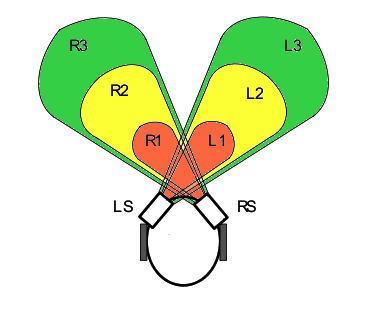
\includegraphics[height=65mm]{../images/ch04/ir_sensor_position.png}
 \caption{Sposób montażu czujników podczerwieni na robocie}
 \label{fig:IRSensorPosition}
\end{figure}

Każdy z czujników składa się z nadajnika i odbiornika podczerwieni a ich
przedział czułości podzielony został na trzy poziomy oznaczone symbolami L1, L2,
L3 dla czujnika lewego i odpowiednio R1, R2, R3 dla czujnika prawego. W chwili
gdy robot znajduje się w ruchu na każdym z czujników jesteśmy w stanie odczytać
wartość odległości od przeszkody, a co za tym idzie możemy kontrolować zachowanie
robota w zależności od poziomu jaki ustalił się na dalmierzach.

\subsection{Algorytm omijania przeszkód}
Algorytm sterujący ruchami robota bazuje więc w całości na danych pomiarowych
otrzymanych z czujników robota. Opisane podejście jest adaptacją metodologii
opisanej w ramach pracy ,,Obstacles Avoidance Method for an Autonomous Mobile
Robot'' \cite{ObstaclesAvoidanceIR}. Algorytm bazuje na prostej maszynie stanów
w której przejścia pomiędzy kolejnymi stanami odbywają się poprzez zmianę poziomów na
czujnikach odległości. Opierając się na takich założeniach, jeżeli oba czujniki
nie wykrywają na swojej drodze przeszkody to robot porusza się z maksymalną
możliwą prędkością. Gdy jeden z czujników wykryje obecność przeszkody na poziomie
 L3 lub/i R3 prędkość poruszania się robota zostanie zmniejszona o połowę. Gdy
 przeszkoda znajdzie się w odległości poziomu L2 lub/i R2 prędkość z
jaką porusza się robot zostanie ustalana na 1/4 prędkości maksymalnej. Jeżeli
natomiast przeszkoda zostanie wykryta na poziomie L1 lub/i R1 robot skręci w
prawo lub lewo w zależności od położenia przeszkody i wyznaczonego celu.

\begin{figure}[hb]
 \centering
 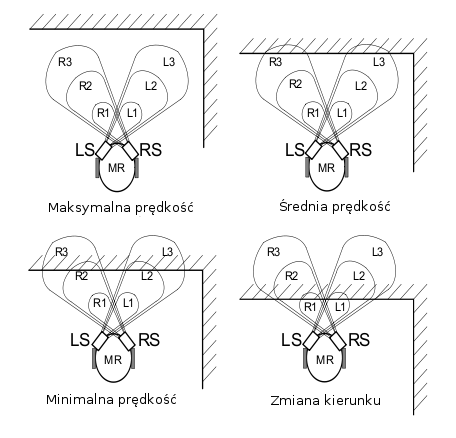
\includegraphics[height=100mm]{../images/ch04/obs_avoid_algorithm.png}
 \caption{Przykładowe sytuacje i definicja reakcji robota}
 \label{fig:IRSensorPosition}
\end{figure}

Tak więc na podstawie odległości od przeszkody robot dostosowuje swoją
prędkość. W chwili gdy robot znajdzie się bezpośrednio przed przeszkodą skręci
on w lewo lub w prawo aby ją ominąć. Szczegółowy opis poszczególnych możliwych
sytuacji oraz rodzaj akcji podejmowanej przez robota jest przedstawiony w
tabeli poniżej. Jedynka w tabeli poniżej oznacza obecność przeszkody na danym
poziomie natomiast zero oznaczać będzie brak przeszkody.
\begin{table}[hb]
\centering
   	\begin{tabular}{ | c | c | c | c | c | c | p{5cm} |} \hline
   		R3 & L3 & R2 & L2 & R1 & L1 & Akcja robota \\ \hline
   		0  & 0  & 0  & 0  & 0  & 0  & Maksymalna prędkość\\ \hline
   		0  & 1  & 0  & 0  & 0  & 0  & Średnia prędkość \\ \hline
   		0  & 1  & 0  & 1  & 0  & 0  & Minimalna prędkość \\ \hline
   		0  & 1  & 0  & 1  & 0  & 1  & Skręt w lewo o $45\,^{\circ}$ \\ \hline 
   		1  & 0  & 0  & 0  & 0  & 0  & Średnia prędkość \\ \hline
   		1  & 0  & 1  & 0  & 0  & 0  & Minimalna prędkość \\ \hline
   		1  & 0  & 1  & 0  & 1  & 0  & Skręt w prawo o $45\,^{\circ}$  \\ \hline
   		1  & 1  & 0  & 0  & 0  & 0  & Średnia prędkość \\ \hline
   		1  & 1  & 1  & 0  & 0  & 0  & Minimalna prędkość \\ \hline
   		1  & 1  & 1  & 0  & 1  & 0  & Skręt w prawo o $45\,^{\circ}$ \\ \hline
   		1  & 1  & 0  & 1  & 0  & 0  & Minimalna prędkość \\ \hline
   		1  & 1  & 0  & 1  & 0  & 1  & Skręt w lewo o $45\,^{\circ}$ \\ \hline 
   		1  & 1  & 1  & 1  & 0  & 0  & Minimalna prędkość \\ \hline 
   		1  & 1  & 1  & 1  & 0  & 1  & Skręt w lewo o $45\,^{\circ}$ \\ \hline 
   		1  & 1  & 1  & 1  & 1  & 0  & Skręt w prawo o $45\,^{\circ}$ \\ \hline 
   		1  & 1  & 1  & 1  & 1  & 1  & Skręt w lewo o $90\,^{\circ}$ \\ \hline
   	\end{tabular}
\caption{Zachowanie robota w zależności od stanu wykrywanego na czujnikach odległości}
\label{ObstacleAvoidTable}
\end{table}\\
Podane w tabeli wartości mają charakter orientacyjny i w przypadku gdy robot ma
wyznaczony cel do którego zmierza kierunki skrętu mogą ulec zmianie. Mogą
również pojawić się dodatkowe zmiany kierunku jazdy umożliwiające odnalezienie
wyznaczonego punktu docelowego. \newpage
\subsection{Implementacja}
W zrealizowanej w ramach pracy magisterskiej implementacji robot, Dark Explorer,
wyposażony został w dwa dalmierze Sharp GP2D12 o efektywnym zasięgu od 10 do 80
cm. Każdy z dalmierzy wyposażony jest w nadajnik i odbiornik IR. Czujnik
GP2D12 samodzielnie dokonuje pomiaru odległości i zwraca go w postaci sygnału
analogowego. Dlatego też, robot wykorzystuje konwerter analogowo-cyfrowy do
przetwarzania wyniku pomiaru otrzymanego z czujnika. Wartość napięcia otrzymana
na wyjściu z konwertera jest za pomocą równania, otrzymanego na podstawie
charakterystyki wyjściowej dalmierza, zamieniana na odległość czujnika od
przeszkody. Na rysunku poniżej przedstawiony został schemat budowy czujnika oraz
wyprowadzeń umożliwiających podłączenie dalmierza.

\begin{figure}[hb]
 \centering
 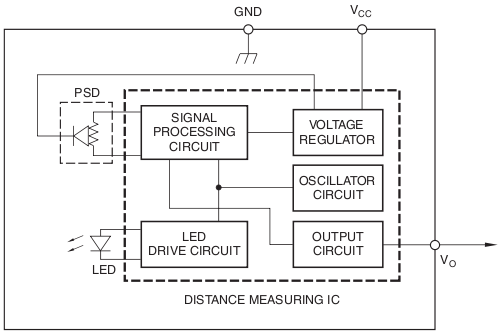
\includegraphics[width=150mm]{../images/ch04/gp2d12_build.png}
 \caption{Budowa czujnika GP2D12 wraz z wyporowadzeniami\cite{GP2D12DataSheet}}
 \label{fig:SharpGP2D12}
\end{figure}

Zgodnie z założeniami algorytmu obszar zasięgu czujników został podzielony na
trzy poziomy. Poziom trzeci zostały wyznaczony w odległości 50 cm, drugi poziom
wyznaczony został w odległości 25 cm, a poziom pierwszy wyznaczony został w
odległości 12 cm od przeszkody. Program zarządzający działaniem robota odczytuje
kolejno dane o odległości otrzymane z czujnika prawego i lewego i kontroluje
zachowanie robota zgodnie z zasadami przedstawionymi w tabeli \ref{ObstacleAvoidTable}.
Z praktycznego punktu widzenia implementacja tego rodzaju algorytmu sprowadza
się do stworzenia tablicy w której przechowywane są prędkości poruszania się każdego z
czterech kół z uwzględnieniem lokalizacji czujnika oraz progu odległości w jakim
znajduje się przeszkoda. 
